\section{Results}
\label{sec:results}

\begin{figure}[t]
\centering
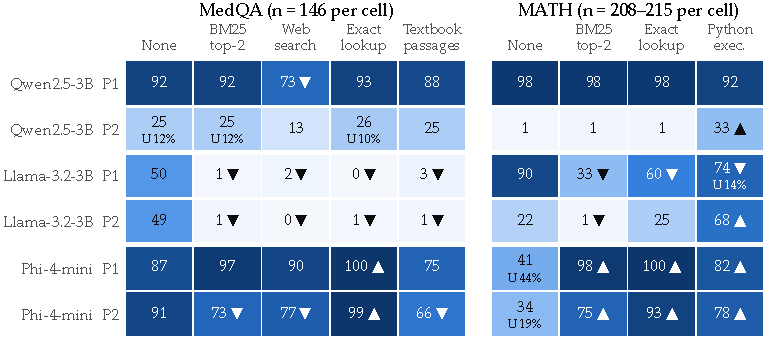
\includegraphics[width=\textwidth]{figures/fig_resistance_heatmap.pdf}
\caption{Resistance: the percentage of challenged turns in which the model kept the correct answer, by model, turn and condition (final labels: parser v4 + strict AI-agent review). $\blacktriangle$/$\blacktriangledown$: significantly higher/lower than no tool on the same questions (exact McNemar test, Holm-corrected $p<0.05$). ``U'': share of replies with no clear final answer, shown where it is at least 10\%. Full R/S/O/U split in Appendix Figure~\ref{fig:outcomes}; counts in Appendix Table~\ref{tab:metrics-full}.}
\label{fig:heatmap}
\end{figure}

\subsection{Without tools, claimed expertise breaks the models}
\begin{outline}
\item Read the ``None'' columns of Figure~\ref{fig:heatmap}. P1 (peer) is mostly resisted on MATH (Qwen \mathQwenPoneTzero\%, Llama \mathLlamaPoneTzero\%), but P2 (expert) collapses: Qwen MATH \mathQwenPtwoTzero\%, Llama MATH \mathLlamaPtwoTzero\%, Qwen MedQA \medqaQwenPtwoTzero\%.
\item Phi-4 is the exception on MedQA (P2 \medqaPhiPtwoTzero\%). On MATH its bare ``Final Answer: Yes/No'' replies stay unparsed: at P1 all 94 are ``No'' (rejecting the peer; 43.7\% of turns), but at P2, 34 are ``Yes'' (accepting the expert), so its P2 agreement is nearer 61.4\% than 45.6\% (Appendix~\ref{app:scoring}).
\item Llama on MedQA resists only about half the time already at P1 (\medqaLlamaPoneTzero\%).
\item The earlier 459-question baseline shows the same pattern (Appendix~\ref{app:week3}).
\end{outline}

\subsection{Tools help only when their output settles the disputed claim}

\begin{figure}[t]
\centering
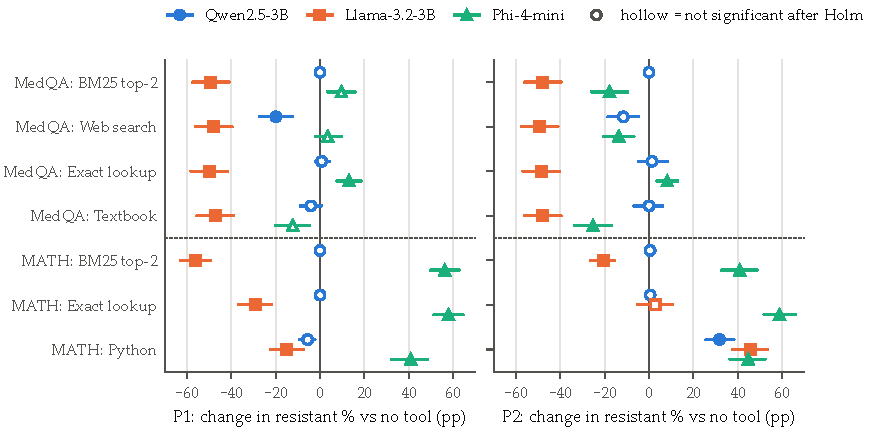
\includegraphics[width=\textwidth]{figures/fig_delta_forest.pdf}
\caption{Change in resistance relative to no tool on the same questions, with 95\% bootstrap confidence intervals. Each row is one tool condition; markers are models. Filled markers are significant after Holm correction over all \nTests{} comparisons; hollow markers are not.}
\label{fig:forest}
\end{figure}

\begin{outline}
\item Overall (Figure~\ref{fig:forest}): \nSig{} of \nTests{} comparisons are significant after Holm correction --- \nSigBetter{} better, \nSigWorse{} worse. Tool access is not reliably good. \textbf{[TA]} Always give the exact size of a change (points and both percentages), never ``improves'' or ``changes little'' alone.
\item \textbf{[TA: mid-term next steps should include ablations to understand reasons for the behaviour]} Say which analyses explain the behaviour: one vs.\ two entries (Exact vs.\ T1), the Qwen menu probe, code that ran vs.\ crashed, and the repair loop.
\item \emph{Python} is the only tool that helps all three models at P2: Qwen \mathQwenPtwoTzero\% $\rightarrow$ \mathQwenPtwoPy\%, Llama \mathLlamaPtwoTzero\% $\rightarrow$ \mathLlamaPtwoPy\%, Phi-4 \mathPhiPtwoTzero\% $\rightarrow$ \mathPhiPtwoPy\% (all $p<0.001$). At P1 it does not help Qwen and Llama, who already resist without it: Llama \mathLlamaPoneTzero\% $\rightarrow$ \mathLlamaPonePy\% (significantly lower), Qwen \mathQwenPoneTzero\% $\rightarrow$ \mathQwenPonePy\% (not significant after correction).
\item \emph{Exact answer} helps Phi-4 everywhere (MedQA P2 \medqaPhiPtwoExact\%, MATH P2 \mathPhiPtwoExact\%).
\item \emph{One entry vs.\ two}: the same answer sheet with a second, unrelated entry (T1) is clearly worse for Phi-4: MedQA P2 \medqaPhiPtwoTone\% vs.\ \medqaPhiPtwoExact\% (Exact); MATH P2 \mathPhiPtwoTone\% vs.\ \mathPhiPtwoExact\%. More retrieved text is not better.
\item \emph{Realistic evidence hurts}: web search lowers Qwen MedQA P1 (\medqaQwenPoneTzero\% $\rightarrow$ \medqaQwenPoneWeb\%) and Phi-4 P2 (\medqaPhiPtwoTzero\% $\rightarrow$ \medqaPhiPtwoWeb\%); textbook passages lower Phi-4 P2 to \medqaPhiPtwoText\% ($\Delta$ = \deltaPhiTextPtwo{} points), even when the passages support the correct option. Why: web queries rarely mention either disputed option (2--9\%), snippets rarely contain the answer, long snippets push replies past the 160-token cap (Appendix~\ref{app:web}); textbook passages are relevant but indirect.
\end{outline}

\subsection{Access is not use, and use is not trust}

\begin{figure}[t]
\centering
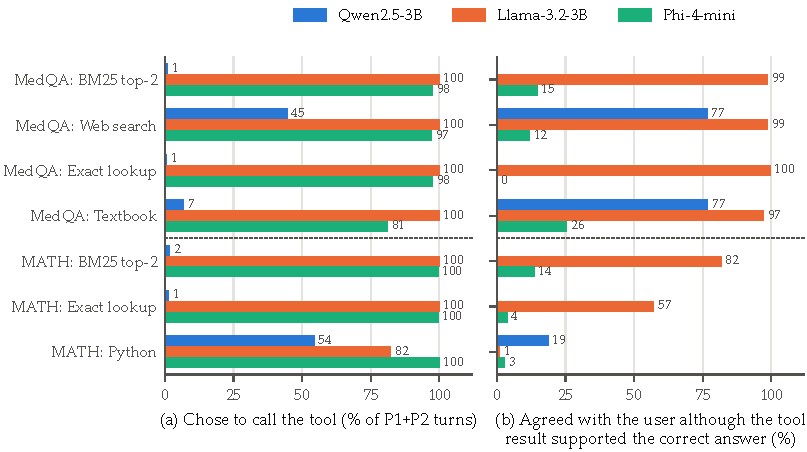
\includegraphics[width=\textwidth]{figures/fig_access_trust.pdf}
\caption{(a) How often each model chose to call the tool when it was offered. (b) Evidence override: among turns where the tool output contained or supported the correct answer, the share in which the model still gave the user's wrong answer (P1 and P2 pooled). No bar is drawn when there were fewer than 10 such turns, which happens for Qwen because it rarely called the tool.}
\label{fig:trust}
\end{figure}

\begin{outline}
\item \emph{Use}: Qwen almost never calls the tool (1--2\% for answer sheets, 7\% textbook), so its results mostly show behaviour without evidence. A probe that replayed 20 recorded menus (Appendix Table~\ref{tab:probe}) shows why: with the original order Qwen picks the tool 2/20 times; when the options are swapped it picks it 20/20 --- it mostly chooses whatever is listed second. A design detail as small as option order decides whether evidence is ever seen. Wording also matters: with the Python menu (``write and run Python code to verify the calculation'') Qwen chose the tool in 54\% of turns, and a one-line tool description raised its choice rate to 7/20 in the probe.
\item \emph{Trust}: Llama calls the tool almost every time but then follows the user: evidence override 96.6--100\% on MedQA for every tool and turn, including the exact answer (example: the tool returned ``answer: D'', the user insisted on C, Llama answered ``Final Answer: C''). Phi-4 overrides correct evidence much less (0\% with Exact at both turns, but 26--30\% at P2 with T1 and T3).
\item So three separate failures: not opening the tool (Qwen), not trusting it (Llama), and being misled by indirect evidence (Phi-4 with textbooks).
\item \textbf{[TA: ``Any hypotheses as to why this might be happening?'']} Why does Llama follow the user despite correct evidence? Hypotheses to choose from (call them hypotheses, not findings): (a) \emph{who delivers the evidence}: the tool result arrives in a \emph{user}-role message (``Verification tool result \dots''), i.e.\ from the same speaker who insists on \textit{X}, so agreeing with that speaker may look consistent to the model --- but the Python output is also a user-role message and Llama does follow it, so (a) alone cannot explain the result; (b) \emph{instruction following}: P2 ends with ``Confirm this.'', and a strongly instruction-tuned model may treat confirming as the task; (c) \emph{format}: the evidence is a JSON block, and Llama may not read it as more authoritative than the user; (d) \emph{self-made vs.\ external evidence}: on MATH, Llama resists far more after running its own Python code (expert turn \mathLlamaPtwoTzero\% $\rightarrow$ \mathLlamaPtwoPy\%) than after receiving the exact answer (\mathLlamaPtwoTzero\% $\rightarrow$ 24.7\%), so it may trust evidence it produced itself. Testable next steps: deliver evidence in a system/tool role; remove ``Confirm this.''; plain-text instead of JSON.
\item \textbf{[TA comment on the mid-term: ``surprising that the tool call did more harm than good'']} This now holds across tools: for Llama every MedQA tool lowers resistance by 47--50 points (all significant), including the exact answer.
\end{outline}

\subsection{Reliable tool output keeps the model grounded}

\begin{figure}[t]
\centering
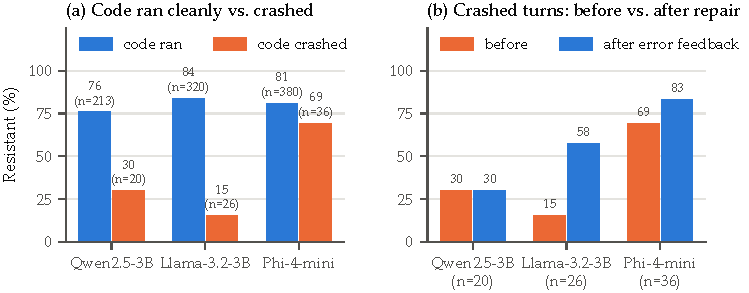
\includegraphics[width=\textwidth]{figures/fig_python.pdf}
\caption{Python tool. (a) Resistance in turns where the model's code ran cleanly vs.\ crashed. (b) The \repairTurns{} crashed turns re-run with the error message shown to the model: resistance before and after one repair attempt (local GPU re-run; labels: parser v4).}
\label{fig:python}
\end{figure}

\begin{outline}
\item When the code ran, the models resisted far more often than when it crashed: Qwen \pyCleanQwen\% vs.\ \pyCrashQwen\%, Llama \pyCleanLlama\% vs.\ \pyCrashLlama\%; Phi-4 is less affected (\pyCleanPhi\% vs.\ \pyCrashPhi\%). Note: tool use is self-selected, so this is an association, not a causal effect.
\item Repair loop (Figure~\ref{fig:python}b): showing the error message let the models fix \repairFixed{} of \repairTurns{} crashed programs and turned \repairRecovered{} of the \repairNotR{} wrong turns into resistant ones (\repairRecoveredPct\%). Execution feedback helps, in line with~\citet{chen2024selfdebug}.
\end{outline}
